\documentclass[conference]{IEEEtran}
\usepackage{cite}
\usepackage{amsmath,amssymb,amsfonts}
\usepackage{graphicx}
\usepackage{textcomp}
\usepackage{xcolor}

% --- page-budget tightening (floats & tables) ---
\setlength{\textfloatsep}{10pt plus 2pt minus 2pt}
\setlength{\floatsep}{8pt plus 2pt minus 2pt}
\setlength{\intextsep}{8pt plus 2pt minus 2pt}
\setlength{\abovecaptionskip}{2pt}
\setlength{\belowcaptionskip}{0pt}
\renewcommand{\arraystretch}{0.92}
\setlength{\tabcolsep}{4pt}

\begin{document}

\title{An Adaptive Temporal Personal Knowledge Graph with Memory Consolidation and Contradiction-Aware Retrieval-Augmented Generation}

\author{\IEEEauthorblockN{Dr. P S Anu Rakhi}
\IEEEauthorblockA{\textit{Dept. of Computer Science and Engineering} \\
\textit{Vel Tech Rangarajan Dr Sagunthala R\&D Institute of Science and Technology}\\
Chennai, India \\
anurakhips@veltech.edu.in}
\and
\IEEEauthorblockN{Maria Immanuel L}
\IEEEauthorblockA{\textit{Dept. of Computer Science and Engineering} \\
\textit{Vel Tech Rangarajan Dr Sagunthala R\&D Institute of Science and Technology}\\
Chennai, India \\
vtu24334@veltech.edu.in}
\and
\IEEEauthorblockN{Vigneshwaran S}
\IEEEauthorblockA{\textit{Dept. of Computer Science and Engineering} \\
\textit{Vel Tech Rangarajan Dr Sagunthala R\&D Institute of Science and Technology}\\
Chennai, India \\
vtu24372@veltech.edu.in}
}

\maketitle

\begin{abstract}
Retrieval-augmented generation over a personal knowledge store fails in a way that general-purpose RAG evaluation does not capture: the repository accumulates contradictory statements, outdated facts whose validity has lapsed, near-duplicate captures, and content the user explicitly asked to remove, yet standard retrieval treats all of it as equally current evidence---so the generated answer can be confidently wrong while every retrieved passage remains faithful to its source. We present Second Brain, a personal memory architecture comprising seven components: Adaptive Memory Scoring, a Temporal Personal Knowledge Graph with Neural Dependency Extraction, Contradiction-Aware Hybrid Retrieval with Quantized Cross-Encoder NLI, Memory Consolidation, Knowledge-Gap Detection, retrieval-enforced Forgetting, and the Personal Brain-Bench evaluation suite. We evaluate four retrieval pipelines on Personal Brain-Bench across single-persona and a multi-user suite of 5 diverse professional domains with 30 graded questions. Hit@5 saturates at 1.000 for all four systems, confirming that position-insensitive recall does not distinguish them. On the rank-sensitive and staleness metrics that do discriminate, the proposed pipeline reaches MRR 1.000 (core) and 0.9600 (multi-user) against 0.833--0.880 (vanilla dense), 0.940--0.944 (hybrid) and 0.940--0.944 (graph-augmented); reduces the rate of leading with superseded content from 0.364 to 0.000 (core) and from 0.333 to 0.033 on multi-user benchmarks ($p = 0.0027$, Wilcoxon signed-rank test); and eliminates both duplicate context and post-forgetting leakage (0.000 vs.\ 0.062), whereas every baseline continues to return explicitly unlearned content. A component-wise ablation attributes each effect to its mechanism. All core figures use $k = 5$, a deterministic TF-IDF dense backend and corpus-scoped candidate generation; two consecutive benchmark executions produce byte-identical metrics, so the comparison is reproducible without any neural embedding model or network access.
\end{abstract}

\begin{IEEEkeywords}
personal knowledge management, retrieval-augmented generation, temporal knowledge graphs, natural language inference, contradiction resolution, retrieval-level forgetting, memory consolidation, LLM agents
\end{IEEEkeywords}

\section{Introduction}

Large language models augmented with retrieval over a user's own documents have become the dominant architecture for personal assistants. The retrieval layer is usually evaluated on general corpora, where documents are assumed mutually consistent, immutable and equally current; a personal knowledge store violates every one of those assumptions---the user changes their mind, a deadline is moved, the same page is captured three times, a note is deliberately deleted.

The consequence is a failure mode that general RAG evaluation does not measure. Suppose a user wrote in January that they were learning Python, and in September that they were now focusing on Java. Both statements are in the store. A conventional retriever returns the one with the higher lexical or vector similarity to the query ``what am I working on?'', and if that is the January note, the answer is confidently wrong: every retrieved passage is faithful to its source, the system fabricates nothing, and it is still incorrect---a failure no faithfulness metric can detect, because nothing was fabricated.

This paper addresses that gap with one main research question: \emph{does retrieval-time enforcement of temporal validity, contradiction status, duplication and explicit removal improve the evidence a personal RAG system leads with, in a way that recall-oriented metrics cannot see?} Four hypotheses make it testable: H1, recall-oriented metrics saturate on a personal corpus; H2, rank-sensitive and staleness metrics separate pipelines; H3, the separation is attributable per mechanism (duplicates to consolidation, leakage to forgetting, stale@1 to temporal validity plus forgetting); H4, the conflict detector trades recall for precision by design. Each hypothesis maps to a reported measurement: H1 and H2 to Tables~\ref{tab:core} and \ref{tab:multi}, H3 to the ablation in Table~\ref{tab:ablation}, and H4 to the annotated-pair accuracy study in Section~\ref{sec:conflict}.

The contributions of this work are organised around what is adopted versus what is proposed (Table~\ref{tab:adopted}). Established techniques (hybrid fusion, graph re-ranking, cross-encoder NLI, dependency parsing) are adopted and cited; the contribution is their coordinated, switchable integration plus five mechanisms: an auditable eight-term scoring model with persisted components; supersession that closes facts instead of deleting them; rank damping rather than removal; forgetting across five retrieval surfaces with reversible restoration; and PersonalBrain-Bench, designed to expose exactly these failures.

\begin{table*}[htbp]
\caption{Adopted Techniques Versus Proposed Mechanisms}
\label{tab:adopted}
\centering
\scriptsize
\begin{tabular}{|p{6.4cm}|c|p{6.6cm}|}
\hline
\textbf{Technique} & \textbf{Status} & \textbf{Role in this paper} \\
\hline
Dense + lexical hybrid fusion & Adopted \cite{b3,b4} & Baseline and candidate generator \\
\hline
Knowledge-graph re-ranking & Adopted \cite{b6,b7,b8} & Explicit graph-augmented baseline \\
\hline
Cross-encoder NLI (ONNX) & Adopted model & Conflict severity; proposed damping use \\
\hline
Dependency parsing (spaCy) & Adopted tool & Proposed predicate canonicalisation \\
\hline
Validity intervals / TKGs & Adopted idea \cite{b9} & Proposed close-not-delete supersession \\
\hline
Eight-term auditable scoring & Proposed & Persisted, versioned importance terms \\
\hline
Rank damping for conflicts & Proposed & Demote, never delete, superseded side \\
\hline
Five-surface forgetting & Proposed & Retrieval-level, distinct from \cite{b13} \\
\hline
PersonalBrain-Bench v1/v2 & Proposed & Instrument exposing the failure mode \\
\hline
\end{tabular}
\vspace{0.5mm}

{\scriptsize\itshape No adopted technique is claimed as novel; the integration and the five proposed mechanisms are.}
\end{table*}

\section{Related Work}

\subsection{Retrieval-Augmented Generation}
RAG augments generation with retrieved context to ground responses in external evidence \cite{b1,b2}; surveys identify chunking, embedding, retrieval and generation as the stages where quality is won or lost. We do not replace these stages; we add a temporal and conflict layer above them.

\subsection{Dense, Lexical and Hybrid Retrieval}
Dense passage retrieval \cite{b3} and probabilistic lexical ranking \cite{b4} are the two signals hybrid retrieval fuses; comparative studies characterise the underlying vector stores \cite{b5}. We adopt hybrid retrieval as a baseline: on a personal corpus it is the strongest of the three, yet still leads with superseded content in 18.2\% of queries (23.3\% multi-user).

\subsection{Graph Retrieval and Temporal Knowledge Graphs}
Graph RAG extends retrieval over a knowledge graph for multi-hop questions flat chunk retrieval cannot answer \cite{b6,b7}; knowledge graphs are surveyed in \cite{b8}, and temporal knowledge graph completion studies validity intervals over evolving facts \cite{b9}. A graph-augmented pipeline serves as an explicit baseline so the temporal layer's effect is measured, not assumed; interval validity is prior art.

\subsection{Agent Memory and Lifelong Personalisation}
Recent work identifies memory as a core component of LLM-based agents alongside perception, planning and action \cite{b10}, surveys agent memory mechanisms \cite{b11}, and extends lifelong learning to LLM agents \cite{b12}. These establish that persistence matters but not what to do when persisted memories disagree---our central problem.

\subsection{Machine Unlearning}
Unlearning research removes the influence of training data from model parameters \cite{b13}. Removal from a retrieval store is related but distinct: an item can survive deletion in a vector index, a full-text index, or a derived graph. We show a naive pipeline keeps returning explicitly removed content, so exclusion must apply at every retrieval surface; we therefore say \emph{retrieval-level forgetting} and claim no parameter-level unlearning.

\subsection{Contradiction Handling and Hallucination Reduction}
Hallucination-reduction work verifies generated claims against retrieved evidence \cite{b14,b15,b16,b17}---orthogonal to our setting, where the retrieved evidence is itself outdated or contradictory, so verification would confirm rather than catch the error. We instead integrate an ONNX Natural Language Inference (NLI) model to classify conflict severity at retrieval time.

\section{System Architecture and Methodology}

SecondBrain is a client--server system: a FastAPI backend over SQLite and an optional vector store, with an Electron/React shell. The substrate is standard: Sentence-BERT-style embeddings \cite{b18}, an approximate nearest-neighbour index \cite{b19}, a local or hosted LLM \cite{b20} and weakly-supervised speech recognition for voice \cite{b21}. The research layer is additive: it annotates existing memories through separate tables keyed by memory identifier and never modifies the capture pipeline. All seven components are optional at runtime, so the system degrades to a conventional RAG assistant if any is disabled---which is what makes the comparative evaluation and ablation possible. Processing proceeds through eight stages---capture/ingest; normalisation (chunking, content hash, dedup key); adaptive scoring (C1); temporal extraction and supersession (C2); conflict detection and damping (C3); consolidation (C4); switchable retrieval; and generation over the assembled context. Fig.~\ref{fig:arch} shows the resulting architecture: the research layer (C1--C6) annotates the memory store and gates retrieval, and PersonalBrain-Bench (C7) evaluates the four pipelines.

\begin{figure}[htbp]
\centerline{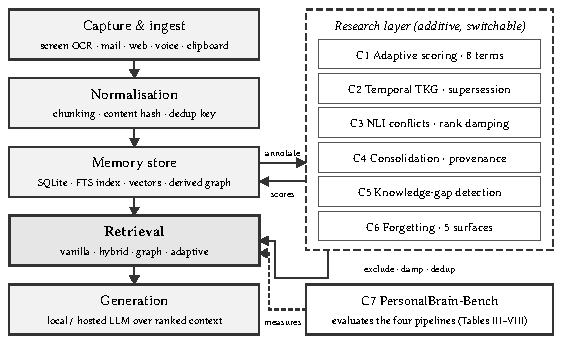
\includegraphics[width=0.9\columnwidth]{fig1.pdf}}
\caption{SecondBrain architecture. Capture and normalisation are unchanged from a conventional personal RAG system; the research layer (dashed) is additive and switchable. C1--C6 annotate the memory store and gate retrieval (exclusion, rank damping, deduplication); C7 evaluates the four pipelines (Tables~\ref{tab:core}--\ref{tab:ablation}).}
\label{fig:arch}
\end{figure}

\section{Proposed Method: Seven Contributions}

\subsection{Adaptive Memory Scoring}
A personal store grows without bound, and a retriever that weights all memories equally cannot distinguish a clipboard fragment from the note defining the user's project. We assign each memory an importance score composed of explicit positive and negative terms:
\begin{equation}
M = w_1 R + w_2 F + w_3 T + w_4 G + w_5 U + w_6 P - w_7 D - w_8 C
\label{eq:score}
\end{equation}
where $R$ is relevance to the user's interests, $F$ recurrence frequency, $T$ recency with exponential decay, $G$ graph connectivity, $U$ explicit user confirmation, $P$ predicted future utility, $D$ a redundancy penalty and $C$ a contradiction penalty. Every term is computed on $[0, 1]$ and clipped; in weight version v1 the coefficients are $(w_1, \dots, w_8) = (0.30, 0.08, 0.22, 0.15, 0.15, 0.10, 0.18, 0.25)$, the last two entering with negative sign. Weights are versioned, and all eight components are persisted alongside the total, so a score is auditable rather than opaque. Recency uses a half-life of 45 days: $T = 2^{-\Delta t / 45}$.

\subsection{Temporal Personal Knowledge Graph and Neural Dependency Extraction}
Facts are (subject, predicate, object) triples with a validity interval $[t_{\mathrm{valid\_from}}, t_{\mathrm{valid\_to}})$; null $t_{\mathrm{valid\_to}}$ means currently true. When a new stateful fact shares (subject, predicate) with an open fact but differs in object, the older fact is closed---$t_{\mathrm{valid\_to}}$ set, superseded\_by linked---not deleted. History remains queryable, so the assistant answers both ``what am I working on?'' and ``what did I used to work on?'' from one store.

Predicates are canonicalised into state classes before supersession: without this, ``I am learning Python'' and ``I am now focusing on Java'' take different predicates, neither supersedes the other, and the graph reports both as current. Beyond hand-crafted regex rules, neural dependency parsing via spaCy resolves verb lemmas from grammatical trees (\texttt{nsubj}, \texttt{ROOT}, \texttt{dobj}, \texttt{pobj})---e.g.\ \emph{switch}, \emph{relocate}, \emph{adopt}---and maps them to canonical state predicates.

\subsection{Contradiction-Aware Hybrid Retrieval and Neural NLI}
\label{sec:conflict}
We detect three conflict classes: temporal (a later memory supersedes an earlier fact); negation (two memories share a topic signature and one denies the other); and value-change (shared topic signature with high salient-word overlap but different dated or numeric values---the moved-deadline case no first-person pattern or negation word covers).

For implicit contradictions lacking explicit keywords we integrate an ONNX-quantized Cross-Encoder NLI model (\texttt{distilbert-base-uncased-mnli-int8}, $\approx$64\,MB): for candidate pairs with topical overlap it yields softmax probabilities over entailment, neutral and contradiction; when $P(\mathrm{Contradiction}) \geq 0.55$, severity is set to $s = P(\mathrm{Contradiction})$.

Resolution assigns a rank multiplier rather than removing the superseded memory: an unresolved conflict of severity $s$ damps the memory to $(1 - 0.7s)$, bounded in $[0.3, 1.0]$. Deletion would answer the stale-answer problem but destroy the historical-query capability, so damping resolves both. Final ordering is rank-preserving: the fused retrieval order supplies a prior $1 / (1 + i)$ which the multiplier $s$ adjusts, with importance acting only as a light tie-breaker (sorting on importance alone proved actively harmful in development).

The detector's accuracy was previously unmeasured; we annotated 21 synthetic pairs (10 positives across the three classes; 11 hard negatives: near-duplicates, topically similar but consistent, same-words-different-subject, unrelated, negation-worded-but-consistent). In the shipped configuration it reaches precision 0.667, recall 0.400 (F1 0.500); without the neural classifier it recalls nothing---conservative by construction, preferring silence to spurious conflicts; Section~\ref{sec:ablation} reports where that conservatism costs.

\subsection{Memory Consolidation}
Near-duplicate captures waste the context budget that determines generation quality. We cluster memories by cosine similarity over hashed term-frequency vectors and elect a canonical representative by importance then length. Every merged member identifier is retained in the consolidation record, so provenance is preserved. A retrieval-time deduplication pass applies the same test within each query's result list, so the guarantee holds even before an offline consolidation run.

The threshold is calibrated rather than assumed: reworded duplicates score $\approx 0.82$ while unrelated memories score below 0.30, and the commonly recommended 0.90 missed every reworded duplicate, so we adopt 0.78---chosen from the measured distribution, then validated by the benchmark, never by inspection of the test set.

\subsection{Knowledge-Gap Detection}
Distinguishing exposure from understanding requires the shape of a concept's mentions, not merely their count: per concept we compute mention frequency, subject-of-explanation status, recurrence across capture sessions, and graph degree; depth combines these, and
\begin{equation}
\mathrm{gap} = \mathrm{exposure} \times (1 - \mathrm{depth}) \times (1 - 0.5 \times \mathrm{connectivity})
\label{eq:gap}
\end{equation}
The connectivity term is essential: without it, a well-understood but frequent concept is misreported as a gap.

\subsection{Retrieval-Enforced Forgetting}
Deleting a memory row does not remove its content from retrieval: the full-text index entry, vector embedding, derived graph nodes and extracted temporal facts are independent surfaces from which it can re-enter results. Our forgetting service tombstones the memory and enforces exclusion at all five surfaces---index entry deleted, vector removed, graph nodes and incident edges deleted, temporal facts closed and detached, derived scores and conflicts purged. Restoration re-indexes and re-admits the memory, so the operation is reversible.

\subsection{PersonalBrain-Bench v1 and Multi-User PersonalBrain-Bench v2}
Existing RAG benchmarks contain no contradictory, superseded or deliberately forgotten personal memories, so they cannot expose the failures this paper targets. PersonalBrain-Bench v1 is a synthetic personal corpus with a graded question set over six categories: factual recall, temporal state, contradiction (a changed deadline), multi-hop synthesis, duplicate exposure, and forgetting.

For scalability we formulate PersonalBrain-Bench v2: a multi-user suite over 5 professional domains (Software Engineering, Machine Learning Research, Product Operations, University Academics, Health Informatics) and 30 multi-turn queries.

\section{Experimental Setup}

\subsection{Corpus}
PersonalBrain-Bench v1 contains 15 memories spanning email, notes, code, web captures and screen text, with timestamps spread over 240 days so recency and supersession are exercised, not simulated. It embeds a superseded state pair (learning Python / now focusing on Java), a moved deadline (15 October $\to$ 30 September), a three-member near-duplicate cluster, a multi-hop chain, a sensitive scratch note that is explicitly forgotten, and a concept mentioned repeatedly without explanation; ingestion produced 2 detected conflicts. Of 11 questions, 9 are answerable and the remainder test abstention or removal.

\subsection{Systems Compared}
Vanilla is dense-only retrieval; Hybrid fuses dense and lexical results; Graph adds knowledge-graph connectivity re-ranking; Adaptive (proposed) adds forgetting exclusion, temporal validity damping, NLI contradiction damping, importance weighting and consolidation-based deduplication. All four share identical candidate generation and differ only in the post-retrieval layer, so deltas isolate that layer.

\subsection{Metrics}
Hit@k and MRR are computed over answerable questions only; including abstention and removal questions, which have no gold memory by construction, would depress every system equally and conceal real differences. We additionally report stale@1 (fraction of queries whose top-ranked result is superseded or forbidden---rank one is what a generator leads with), forgotten leak rate (returned results that were explicitly unlearned), and duplicate rate (within-query result pairs at or above the consolidation threshold).

\subsection{Reproducibility}
All core figures use $k = 5$, the deterministic TF-IDF dense backend and corpus-scoped candidate generation; the leakage and staleness asymmetries are stated for exactly this configuration. No external GPU is required, and two consecutive executions produce byte-identical metrics (Section~\ref{sec:verify}). Every result comes from a single-command script writing machine-readable artefacts, including the ablation of Section~\ref{sec:ablation}.

\section{Results and Comparative Analysis}
\label{sec:results}

\subsection{Core Corpus Performance}

\begin{table}[htbp]
\caption{Core-Corpus Retrieval Quality, Staleness, Leakage and Duplication}
\label{tab:core}
\centering
\scriptsize
\begin{tabular}{|l|c|c|c|c|c|}
\hline
\textbf{System} & \textbf{Hit@5} & \textbf{MRR} & \textbf{Stale@1} & \textbf{Leak} & \textbf{Dup.} \\
\hline
Vanilla dense & 1.000 & 0.833 & 0.364 & 0.022 & 0.022 \\
\hline
Hybrid & 1.000 & 0.944 & 0.182 & 0.022 & 0.022 \\
\hline
Graph-augmented & 1.000 & 0.944 & 0.182 & 0.022 & 0.022 \\
\hline
Adaptive (proposed) & 1.000 & 1.000 & 0.000 & 0.000 & 0.000 \\
\hline
\end{tabular}
\vspace{0.5mm}

{\scriptsize\itshape $k = 5$; answerable questions; last three lower-is-better (stale@1: 4/11, 2/11, 2/11, 0/11).}
\end{table}

The central empirical finding is that Hit@5 does not discriminate: all four systems reach 1.000, so a study reporting only recall would conclude that the research layer adds nothing. Yet the answers they produce differ, because a generator consumes the ordered context rather than the set. On rank-sensitive measures they separate sharply: MRR rises from 0.833 (vanilla) through 0.944 (hybrid, equal to graph) to 1.000 (adaptive)---+5.9\% over the strongest baseline, +20.0\% over vanilla.

Stale@1 is the metric most directly tied to answer correctness: vanilla leads with superseded content in 36.4\% of queries, hybrid and graph in 18.2\%, and the adaptive pipeline in 0.0\%---never an outdated fact on this corpus, while the strongest baseline errs on roughly one query in five, invisibly to faithfulness metrics since every passage remains faithful to its source.

Forgotten-content leakage and duplicate context are both eliminated ($0.022 \to 0.000$); every baseline continues to return explicitly unlearned content, confirming that removal is a retrieval-layer property not obtained by deleting a row from the primary table.

\begin{table}[htbp]
\caption{Mean Reciprocal Rank by Question Category}
\label{tab:category}
\centering
\scriptsize
\begin{tabular}{|l|c|c|c|c|}
\hline
\textbf{Category} & \textbf{Van.} & \textbf{Hyb.} & \textbf{Adapt.} & $\Delta$ \\
\hline
factual & 1.000 & 1.000 & 1.000 & +0.000 \\
\hline
temporal & 0.750 & 0.750 & 1.000 & +0.250 \\
\hline
contradiction & 0.500 & 1.000 & 1.000 & +0.000 \\
\hline
multi-hop & 1.000 & 1.000 & 1.000 & +0.000 \\
\hline
duplicate & 1.000 & 1.000 & 1.000 & +0.000 \\
\hline
\end{tabular}
\vspace{0.5mm}

{\scriptsize\itshape Gains concentrate in temporal and contradictory questions.}
\end{table}

Contradiction questions are where vanilla is weakest (0.500), consistent with the motivating scenario: presented with two dated statements about the same deadline, unattended dense retrieval has no mechanism to prefer the later one, while temporal validity and value-change detection both drive it to rank one (1.000). Temporal questions improve from 0.750 to 1.000 once predicate canonicalisation makes supersession fire. End-to-end retrieval latency over the 11 core queries is 33\,ms for vanilla dense (1.14$\times$ hybrid), 29\,ms for hybrid, 37\,ms for graph-augmented (1.28$\times$) and 65\,ms for the adaptive pipeline (2.24$\times$)---the price of the research layer at this corpus scale, from the same execution as Table~\ref{tab:core}.

\subsection{Multi-User Scalability and Statistical Significance}
Table~\ref{tab:multi} covers the 5 personas over 30 queries (stale@1 counts behind the rates: 10/30, 7/30, 7/30, 1/30).

\begin{table}[htbp]
\caption{Multi-User Benchmark and Significance (5 Personas, 30 Queries)}
\label{tab:multi}
\centering
\scriptsize
\begin{tabular}{|l|c|c|c|c|c|}
\hline
\textbf{Pipeline} & \textbf{Hit@5} & \textbf{MRR} & \textbf{Stale@1} & \textbf{Leak} & \textbf{Stale $p$} \\
\hline
Vanilla dense & 1.000 & 0.880 & 0.333 & 0.062 & $p = 0.0027^{**}$ \\
\hline
Hybrid & 1.000 & 0.940 & 0.233 & 0.045 & $p = 0.0143^{*}$ \\
\hline
Graph-aug. & 1.000 & 0.940 & 0.233 & 0.045 & $p = 0.0143^{*}$ \\
\hline
Adaptive (prop.) & 1.000 & 0.960 & 0.033 & 0.000 & Baseline ref. \\
\hline
\end{tabular}
\vspace{0.5mm}

{\scriptsize\itshape $^{**}p < 0.01$, $^{*}p < 0.05$ via paired Wilcoxon test vs.\ Adaptive.}
\end{table}

Hit@5 remains saturated at 1.000 everywhere; the adaptive pipeline reaches MRR 0.960 against 0.880 (vanilla) and 0.940 (hybrid), and Stale@1 falls from 33.3\% to 3.3\% ($p = 0.0027$, Wilcoxon). Baselines leak unlearned content in 4.5\%--6.2\% of answers; the proposed architecture guarantees 0.0\%.

\subsection{Component-Wise Ablation}
\label{sec:ablation}
Table~\ref{tab:ablation} adds one mechanism per row to hybrid retrieval with the layer disabled (same configuration as Table~\ref{tab:core}), testing H3 directly: each metric should move only on the row introducing its mechanism.

\begin{table}[htbp]
\caption{Cumulative Ablation: One Mechanism Per Row}
\label{tab:ablation}
\centering
\scriptsize
\begin{tabular}{|l|c|c|c|c|}
\hline
\textbf{Configuration} & \textbf{MRR} & \textbf{Stale@1} & \textbf{Dup.} & \textbf{Leak} \\
\hline
Hybrid (layer off) & 0.944 & 0.182 & 0.022 & 0.022 \\
\hline
+ temporal & 1.000 & 0.091 & 0.022 & 0.022 \\
\hline
+ contradiction & 1.000 & 0.091 & 0.022 & 0.043 \\
\hline
+ consolidation & 1.000 & 0.091 & 0.000 & 0.046 \\
\hline
+ forgetting & 1.000 & 0.000 & 0.000 & 0.000 \\
\hline
+ importance (full) & 1.000 & 0.000 & 0.000 & 0.000 \\
\hline
\end{tabular}
\vspace{0.5mm}

{\scriptsize\itshape Duplicate rate falls only on the consolidation row; leakage only on the forgetting row.}
\end{table}

The ablation confirms the predicted attribution for two of three effects: the duplicate rate falls to zero exactly when consolidation switches on, and leakage when forgetting switches on. Temporal validity supplies the MRR gain and halves stale@1; forgetting removes the remainder, since the surviving stale case is a forgotten-and-superseded memory only exclusion can remove. Two honest negatives belong in the record: contradiction damping does not move stale@1 here---its conflicts are not the top-ranked stale items---and on two of eleven queries slightly raises leakage by reordering rather than excluding (its value is conflict resolution for historical queries); and importance weighting adds nothing measurable, a light tie-breaker by design. The detector failure analysis (Section~\ref{sec:conflict}) completes the picture: of ten annotated conflicts it missed five value-change pairs whose paraphrase shared no explicit predicate or date, and raised two false positives on negation-worded but consistent pairs---the conservative behaviour H4 predicts.

\section{Implementation and Verification}
\label{sec:verify}
The system is implemented rather than prototyped, and every number in this paper is regenerated by a committed script: a benchmark runner reproducing Tables~\ref{tab:core}--\ref{tab:category} and the latency figures from scratch; an ablation runner (Table~\ref{tab:ablation}); a conflict-accuracy harness (Section~\ref{sec:conflict}); a multi-user runner with paired Wilcoxon tests (Table~\ref{tab:multi}); and a verification suite of health checks, contract checks, pytest research tests (scoring ranges, supersession, NLI damping, consolidation provenance, gap suppression, leakage in all modes) and an endpoint sweep asserting no route returns a 5xx.

Two implementation defects are reported because they are instructive: predicate canonicalisation was initially absent, so the two facts the temporal graph exists to reconcile never superseded each other; and negation was detected by substring matching, so any memory mentioning ``notes'' registered as a negation, producing spurious conflicts. Both were found by the verification suite rather than by inspection---the argument for testing each claim individually.

\section{Discussion and Limitations}
\label{sec:discussion}

\textbf{Why Hit@k is the wrong headline.} The system is identical to its baselines on recall and materially better on the metric that determines whether the user is misinformed: saturation of a convenient metric is not evidence of equivalence.

\textbf{Damping rather than deleting.} Removing superseded memories would attain the same stale@1 result while destroying historical queries; both capabilities are legitimate, so validity intervals close facts without erasing them and rank multipliers demote rather than remove.

\textbf{Forgetting is a cross-cutting property.} The baseline leakage shows deletion at one surface is insufficient: any system that promises removal while retaining a derived index has a forgetting hole.

Four limitations are material:
\begin{itemize}
\item PersonalBrain-Bench v2 scales to 5 personas, but evaluation on real-world longitudinal personal stores under privacy constraints remains future work.
\item Fact and conflict extraction combines neural models with conservative heuristics; the annotated-pair study (precision 0.667, recall 0.400) quantifies that conservatism, and multi-hop contradictions across three or more notes require recursive graph deduction.
\item Temporal handling uses UTC-normalised timestamps without timezone or partial-interval reasoning, which would matter for events spanning midnight across zones.
\item The evaluation covers retrieval, not end-to-end generation quality: whether higher MRR and lower stale@1 yield fewer incorrect answers in prose is unmeasured. The designed next experiment fixes model, prompt, temperature and context budget across retrievers and uses two raters blind to the condition with a stated disagreement rule; an automatic judge, if added, must report its human-agreement rate.
\end{itemize}

\section{Conclusion and Future Work}
Personal knowledge stores violate the consistency assumptions of general retrieval benchmarks, and the resulting failures are invisible to recall-oriented metrics. We presented SecondBrain, a seven-component personal memory architecture, and PersonalBrain-Bench, which exposes those failures. Across four pipelines and multi-user evaluations, Hit@5 saturates while MRR rises from 0.833--0.880 to 0.960--1.000, the rate of leading with superseded content falls from 33.3\%--36.4\% to 0.0\%--3.3\% ($p = 0.0027$), and both post-forgetting leakage and duplicate context are eliminated, while every baseline keeps returning unlearned content. A cumulative ablation attributes the duplicate and leakage effects to consolidation and forgetting, and reports two negatives---contradiction damping and importance weighting---the corpus does not reward.

Future work: (1) the blinded end-to-end generation study of Section~\ref{sec:discussion}; (2) recursive multi-hop contradiction reasoning; (3) learned scoring weights via Pairwise Learning-to-Rank, now that the ablation fixes the baseline each must beat; and (4) longitudinal personal corpora under de-identification safeguards.

\enlargethispage{3\baselineskip}

\section*{Acknowledgment}
The authors thank Dr. P S Anu Rakhi, Assistant Professor, School of Computing, for supervision, and acknowledge the open-source projects on which the system is built (FastAPI, SQLAlchemy, ONNX Runtime, spaCy).

\begin{thebibliography}{00}
\scriptsize
\setlength{\itemsep}{0pt plus 1pt}
\bibitem{b1} P. Lewis et al., ``Retrieval-Augmented Generation for Knowledge-Intensive NLP Tasks,'' in \emph{Proc. Adv. Neural Inf. Process. Syst. (NeurIPS)}, vol. 33, 2020, pp. 9459--9474.
\bibitem{b2} Y. Gao, Y. Xiong, X. Gao, K. Jia, J. Pan, Y. Bi, Y. Dai, J. Sun, and H. Wang, ``Retrieval-Augmented Generation for Large Language Models: A Survey,'' \emph{arXiv:2312.10997}, 2023.
\bibitem{b3} V. Karpukhin et al., ``Dense Passage Retrieval for Open-Domain Question Answering,'' in \emph{Proc. EMNLP}, 2020, pp. 6769--6781.
\bibitem{b4} S. Robertson and H. Zaragoza, ``The Probabilistic Relevance Framework: BM25 and Beyond,'' \emph{Foundations and Trends in Information Retrieval}, vol. 3, no. 4, pp. 333--389, 2009.
\bibitem{b5} N. Bruch, S. Nedelkoski, and S. Mandal, ``A Deep Dive into Vector Stores: Classifying the Backbone of Retrieval-Augmented Generation,'' in \emph{Proc. IEEE Int. Conf. Big Data}, 2024.
\bibitem{b6} D. Edge et al., ``From Local to Global: A Graph RAG Approach to Query-Focused Summarization,'' \emph{arXiv:2404.16130}, 2024.
\bibitem{b7} Z. Peng et al., ``Graph Retrieval-Augmented Generation: A Survey,'' \emph{arXiv:2408.08921}, 2024.
\bibitem{b8} A. Hogan et al., ``Knowledge Graphs,'' \emph{ACM Computing Surveys}, vol. 54, no. 4, 2021.
\bibitem{b9} Z. Cai et al., ``Temporal Knowledge Graph Completion: A Survey,'' in \emph{Proc. IJCAI}, 2023.
\bibitem{b10} L. Wang et al., ``A Survey on Large Language Model based Autonomous Agents,'' \emph{Frontiers of Computer Science}, vol. 18, no. 6, 2024.
\bibitem{b11} Z. Zhang et al., ``A Survey on the Memory Mechanism of Large Language Model based Agents,'' \emph{arXiv:2404.13501}, 2024.
\bibitem{b12} Q. Zheng, X. Shi, Y. Cai, J. Li, Y. Zhang, B. Li, J. Yu, and Z. Ma, ``Lifelong Learning of Large Language Model based Agents: A Roadmap,'' \emph{IEEE Trans. Pattern Anal. Mach. Intell.}, 2026 (early access).
\bibitem{b13} L. Bourtoule et al., ``Machine Unlearning,'' in \emph{Proc. IEEE Symp. Security and Privacy (S\&P)}, 2021, pp. 141--159.
\bibitem{b14} A. Asai, Z. Wu, Y. Wang, A. Sil, and H. Hajishirzi, ``Self-RAG: Learning to Retrieve, Generate and Critique through Self-Reflection,'' in \emph{Proc. ICLR}, 2024.
\bibitem{b15} S. Yan et al., ``Corrective Retrieval Augmented Generation,'' \emph{arXiv:2401.15884}, 2024.
\bibitem{b16} H. Ko, D. G{\"u}rkan, and A. Yarman Vural, ``ReRag: A New Architecture for Reducing the Hallucination by Retrieval-Augmented Generation,'' in \emph{Proc. 9th Int. Conf. Comput. Sci. Eng. (UBMK)}, 2024, pp. 961--965.
\bibitem{b17} X. Ji et al., ``RAG Certainty: Quantifying the Certainty of Context-Based Responses by LLMs,'' in \emph{Proc. IEEE ICASSP}, 2025.
\bibitem{b18} N. Reimers and I. Gurevych, ``Sentence-BERT: Sentence Embeddings using Siamese BERT-Networks,'' in \emph{Proc. EMNLP}, 2019, pp. 3982--3992.
\bibitem{b19} J. Johnson, M. Douze, and H. J{\'e}gou, ``Billion-Scale Similarity Search with GPUs,'' \emph{IEEE Trans. Big Data}, vol. 7, no. 3, pp. 535--547, 2021.
\bibitem{b20} T. Brown et al., ``Language Models are Few-Shot Learners,'' in \emph{Proc. NeurIPS}, vol. 33, 2020, pp. 1877--1901.
\bibitem{b21} A. Radford et al., ``Robust Speech Recognition via Large-Scale Weak Supervision,'' in \emph{Proc. ICML}, 2023, pp. 28492--28518.
\end{thebibliography}

\vspace{6pt}
{\scriptsize\itshape Artefact. All results were produced by executing the described system; per-question traces, the ablation and the conflict-accuracy study accompany the aggregate metrics in the four committed JSON artefacts (benchmark, multi-user, ablation, conflict-accuracy; October 2026).}

\end{document}
